\section{Cost Analysis and Comparison}
\label{sec:cost-analysis}

The stereographic block encoding of
Section~\ref{sec:block-encoding} removes the normalization
factor $\alpha \geq \|H\|$ from the quantum circuit.  But
removing a cost from one column of the ledger does not make it
disappear---it reappears elsewhere, shifting from coherent
circuit depth into classical sampling overhead.

The depth advantage is immediate from the construction:
the stereographic block encoding~\eqref{eq:stereo-block} uses
a single ancilla qubit and does not require knowledge of
$\|H\|$, so the circuit depth depends only on the degree $d$
of the rational approximation.  In the standard approach, by
contrast, the depth scales as $\mathcal{O}(d \cdot \|H\|)$
after accounting for the subnormalization factor, so the depth
saving from stereographic encoding is a multiplicative factor
of $\|H\|$.  For operators with large norm---unbounded spectra,
poorly conditioned systems, or Hamiltonians whose norm grows
with system size---this saving can be substantial.

The saving is not free.  The stereographic decoding
formula~\eqref{eq:decoding} recovers the encoded value $z$ from
the ratio $\langle\PauliX\rangle/(1 - \langle\PauliZ\rangle)$,
and as $r \to \infty$ the denominator
$1 - \langle\PauliZ\rangle \to 0$: the Bloch sphere becomes
increasingly compressed near the north pole, amplifying
measurement noise.  A first-order error propagation (see
Appendix~\ref{app:proofs}) shows that if each Pauli expectation
is estimated with precision $\delta$, the decoded value
$\hat{z}$ satisfies
\begin{equation}
	|\hat{z} - z| \leq \frac{(1+r^2)(1+r)}{2}\,\delta.
	\label{eq:error-bound}
\end{equation}

The error amplification factor grows as $r^3$ for large $r$:
the numerator measurement contributes $\mathcal{O}(r^2)$ and the
denominator measurement $\mathcal{O}(r^3)$.  Since each Pauli
expectation estimated from $N$ shots has precision
$\delta = \mathcal{O}(1/\sqrt{N})$, achieving absolute precision
$|\hat{z} - z| \leq \epsilon$ requires
\begin{equation}
	N = \mathcal{O}\!\left(\frac{(1+r^2)^2(1+r)^2}{\epsilon^2}\right) = \mathcal{O}\!\left(\frac{r^6}{\epsilon^2}\right) \quad \text{for } r \gg 1.
	\label{eq:shot-count}
\end{equation}
For \emph{relative} precision
$|\hat{z}/z - 1| \leq \epsilon_{\mathrm{rel}}$, the scaling
improves to
\begin{equation}
	N = \mathcal{O}\!\left(\frac{r^4}{\epsilon_{\mathrm{rel}}^2}\right) \quad \text{for } r \gg 1,
	\label{eq:shot-count-rel}
\end{equation}
since the relative error bound is
$|\delta z/z| \leq (1+r^2)(1+r)/(2r)\,\delta$, which grows as
$r^2$ rather than $r^3$.  The crucial point is that the overhead
is \emph{polynomial} in $r$, not exponential: large eigenvalues
are expensive to decode, but not catastrophically so.

\textit{Eigenvalue inversion as a case study.}
\label{subsec:inversion-example}
The depth-versus-sampling tradeoff is best appreciated through
a concrete example.  Eigenvalue inversion,
$f(\lambda) = 1/\lambda$, is central to quantum linear systems
algorithms~\cite{HHL2009,ChildsWiebe2012} and is a natural
testbed for stereographic QSP because $1/\lambda$ diverges as
$\lambda \to 0$---precisely the kind of unbounded function that
standard QSP cannot realize directly.

In the standard framework, one normalizes $H \to H/\alpha$ with
$\alpha \geq \|H\|$, then approximates $f(a) = 1/(\alpha a)$
by a bounded polynomial $P(a)$ satisfying $|P(a)| \leq 1$.
Since $1/a$ diverges at $a = 0$, the polynomial can only
approximate it for $|a| \geq \kappa^{-1}$, where
$\kappa = \alpha/\lambda_{\min}$ is the condition number, giving
degree $\mathcal{O}(\kappa \log(1/\epsilon))$ and circuit depth
$\mathcal{O}(\alpha\kappa\log(1/\epsilon))$.

In the stereographic framework, each eigenvalue $\lambda_j$
enters as the signal $r = \lambda_j$, and the decoded output is
$f(\lambda_j) = P(\tilde\lambda_j)/Q(\tilde\lambda_j)$ with
$\tilde\lambda_j = \lambda_j/\sqrt{1+\lambda_j^2}$.  The target
in the bounded variable is
\begin{equation}
	\frac{P(a)}{Q(a)} = \frac{1}{r} = \frac{\sqrt{1-a^2}}{a},
	\label{eq:inversion-target}
\end{equation}
where $a = \tilde\lambda = \lambda/\sqrt{1+\lambda^2}$.  No
normalization constant $\alpha$ appears: the QSP circuit depth
depends only on the approximation degree $d$, not on $\|H\|$.
Figure~\ref{fig:target-gallery} demonstrates this on four
representative target functions: eigenvalue inversion $1/r$,
the Lorentzian $1/(1+r^2)$, the inverse square root
$1/\sqrt{1+r^2}$, and the Gaussian $e^{-r^2}$.  In each case,
the decoded ratio $P(\tilde{r})/Q(\tilde{r})$ (top row) tracks
the exact target increasingly well as the QSP degree~$d$
increases.  The pointwise error (bottom row,
logarithmic scale) reveals the spatial structure of the
approximation: for $1/r$, errors are concentrated at small $r$
where the target diverges; for the bounded targets, errors are
spread more uniformly.  Eigenvalue inversion is the most
favorable case---$1/r = \cot(\arctan(1/r))$ coincides exactly
with the $d = 2$ base case, so already at low degree the
approximation achieves errors below $10^{-7}$.  The bounded
targets require higher degree for comparable accuracy, with
convergence that is algebraic rather than exponential because the
stereographic map introduces branch points at $\tilde{r} = \pm 1$
(corresponding to $r \to \infty$).

\begin{figure*}[tp]
	\centering
	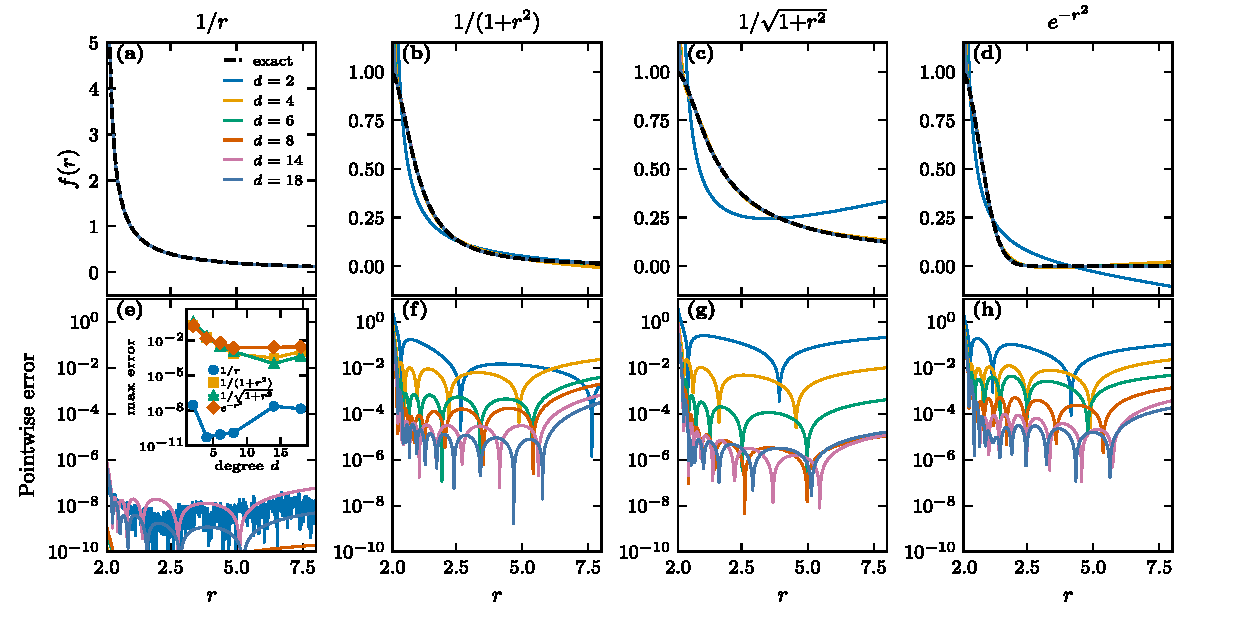
\includegraphics[width=\textwidth]{figures/target_gallery.pdf}
	\caption{Stereographic QSP approximation of four target functions. \emph{Top row}~(a--d): decoded rational functions $P(\tilde{r})/Q(\tilde{r})$ (colored lines, one color per QSP degree~$d$; see legend in~(a)) compared to the exact target (dashed black). All approximations improve systematically with increasing degree. \emph{Bottom row}~(e--h): pointwise error $|f_d(r) - f(r)|$ on a logarithmic scale. For eigenvalue inversion (a,~e), errors are below $10^{-7}$ even at low degree because the $d=2$ base case already captures $1/r$. For the bounded targets (b--d, f--h), the error decreases with degree but more slowly, reflecting the branch point at $\tilde{r} = \pm 1$. \emph{Inset} in~(e): maximum approximation error on the fitting interval versus QSP degree~$d$ for all four targets, showing that eigenvalue inversion converges fastest while bounded targets converge more slowly.}
	\label{fig:target-gallery}
\end{figure*}

For eigenvalue inversion on an operator with condition number
$\kappa$ and $\|H\| = \alpha$, the standard approach requires
circuit depth
$\mathcal{O}(\alpha\kappa\log(1/\epsilon))$---the factor
of~$\alpha$ arising from normalization---while the stereographic
approach has depth $\mathcal{O}(d)$ independent of $\|H\|$, at
the cost of a measurement overhead scaling as
$\mathcal{O}(\lambda_{\max}^6/\epsilon^2)$ for absolute
precision~$\epsilon$.  For operators where $\|H\|$ is large but
the desired eigenvalues are moderate, the depth saving can be
substantial.  Table~\ref{tab:cost-comparison} collects the full
comparison.

\begin{table*}[t]
	\caption{Cost comparison of standard, stereographic, and generalized QSP approaches for implementing a function $f(\lambda)$ of the eigenvalues of a Hermitian operator $H$. Here $\alpha = \|H\|$, $\kappa$ is the condition number, $d$ is the polynomial degree, and $r = \max_j |\lambda_j|$ is the maximum eigenvalue magnitude.}
	\label{tab:cost-comparison}
	\begin{ruledtabular}
		\begin{tabular}{llll}
			                     & Standard QSP/QSVT                   & Stereographic QSP                     & GQSP~\cite{MotlaghWiebe2023}              \\
			\hline
			Output constraint    & $|P(a)| \leq 1$ on $[-1,1]$         & $|P(\rtilde)|^2 + |Q(\rtilde)|^2 = 1$ & $|P(e^{i\theta})| \leq 1$ on $\mathbb{T}$ \\
			Output range         & Bounded                             & Unbounded (rational)                  & Bounded                                   \\
			Circuit depth        & $\mathcal{O}(d \cdot \alpha)$       & $\mathcal{O}(d)$                      & $\mathcal{O}(d)$                          \\
			Ancilla qubits       & $\geq 1$ (implementation-dependent) & $1$                                   & $1$                                       \\
			Normalization        & Required ($\alpha \geq \|H\|$)      & Not required                          & Required ($\alpha \geq \|H\|$)            \\
			Sampling cost        & $\mathcal{O}(1/\epsilon^2)$         & $\mathcal{O}(r^6/\epsilon^2)$         & $\mathcal{O}(1/\epsilon^2)$               \\
			Input domain         & $a \in [-1,1]$                      & $r \in [0,\infty)$                    & $e^{i\theta} \in \mathbb{T}$              \\
			Eigenbasis knowledge & Not required                        & Required                              & Not required                              \\
			Polynomial parity    & Required                            & Required                              & Not required                              \\
		\end{tabular}
	\end{ruledtabular}
\end{table*}

The tradeoff between coherent depth and sampling cost identifies
a natural regime for stereographic QSP: depth-limited devices
where circuit depth is the primary bottleneck, so that saving a
factor of~$\alpha$ in depth outweighs the increased sampling
cost; operators whose eigenvalues of interest satisfy
$r = \mathcal{O}(1)$, where the sampling overhead remains
$\mathcal{O}(1/\epsilon^2)$---the same as standard QSP;
structured Hamiltonians with a known eigenbasis; and genuinely
unbounded target functions ($1/\lambda$, $\lambda$,
$\tan\lambda$) that standard QSP can only approximate after
truncation.  For large eigenvalues $r \gg 1$, the
$\mathcal{O}(r^6/\epsilon^2)$ sampling cost becomes
prohibitive, and standard QSP---which pays
$\mathcal{O}(\alpha)$ coherently but has constant sampling
cost---is preferable.  We discuss the relationship to standard QSP/QSVT and generalized QSP in more detail in Section~\ref{sec:discussion}.
